\section{Technique Knowledge Graph}
\label{sec:tkg}

\subsection{TKG design}

The TKG should take a hierarchical (two-layer) design, namely, system entity (and action) level and TTP level. On system entity level, the TKG looks just like many sub-graphs(TPG) of Provenance Graph.  Every sub-graph represents a TTP and make up the TTP-level TKG. Every TTP node should have one or more inputs and outputs. And we can use these inputs and outputs connect TTPs.


\subsubsection{Layer 1: kill chain layer}

\subsubsection{Layer 2: TTP representation layer}

\subsection{Initing the TKG – The Workflow:
}

\begin{figure}
    \centering
    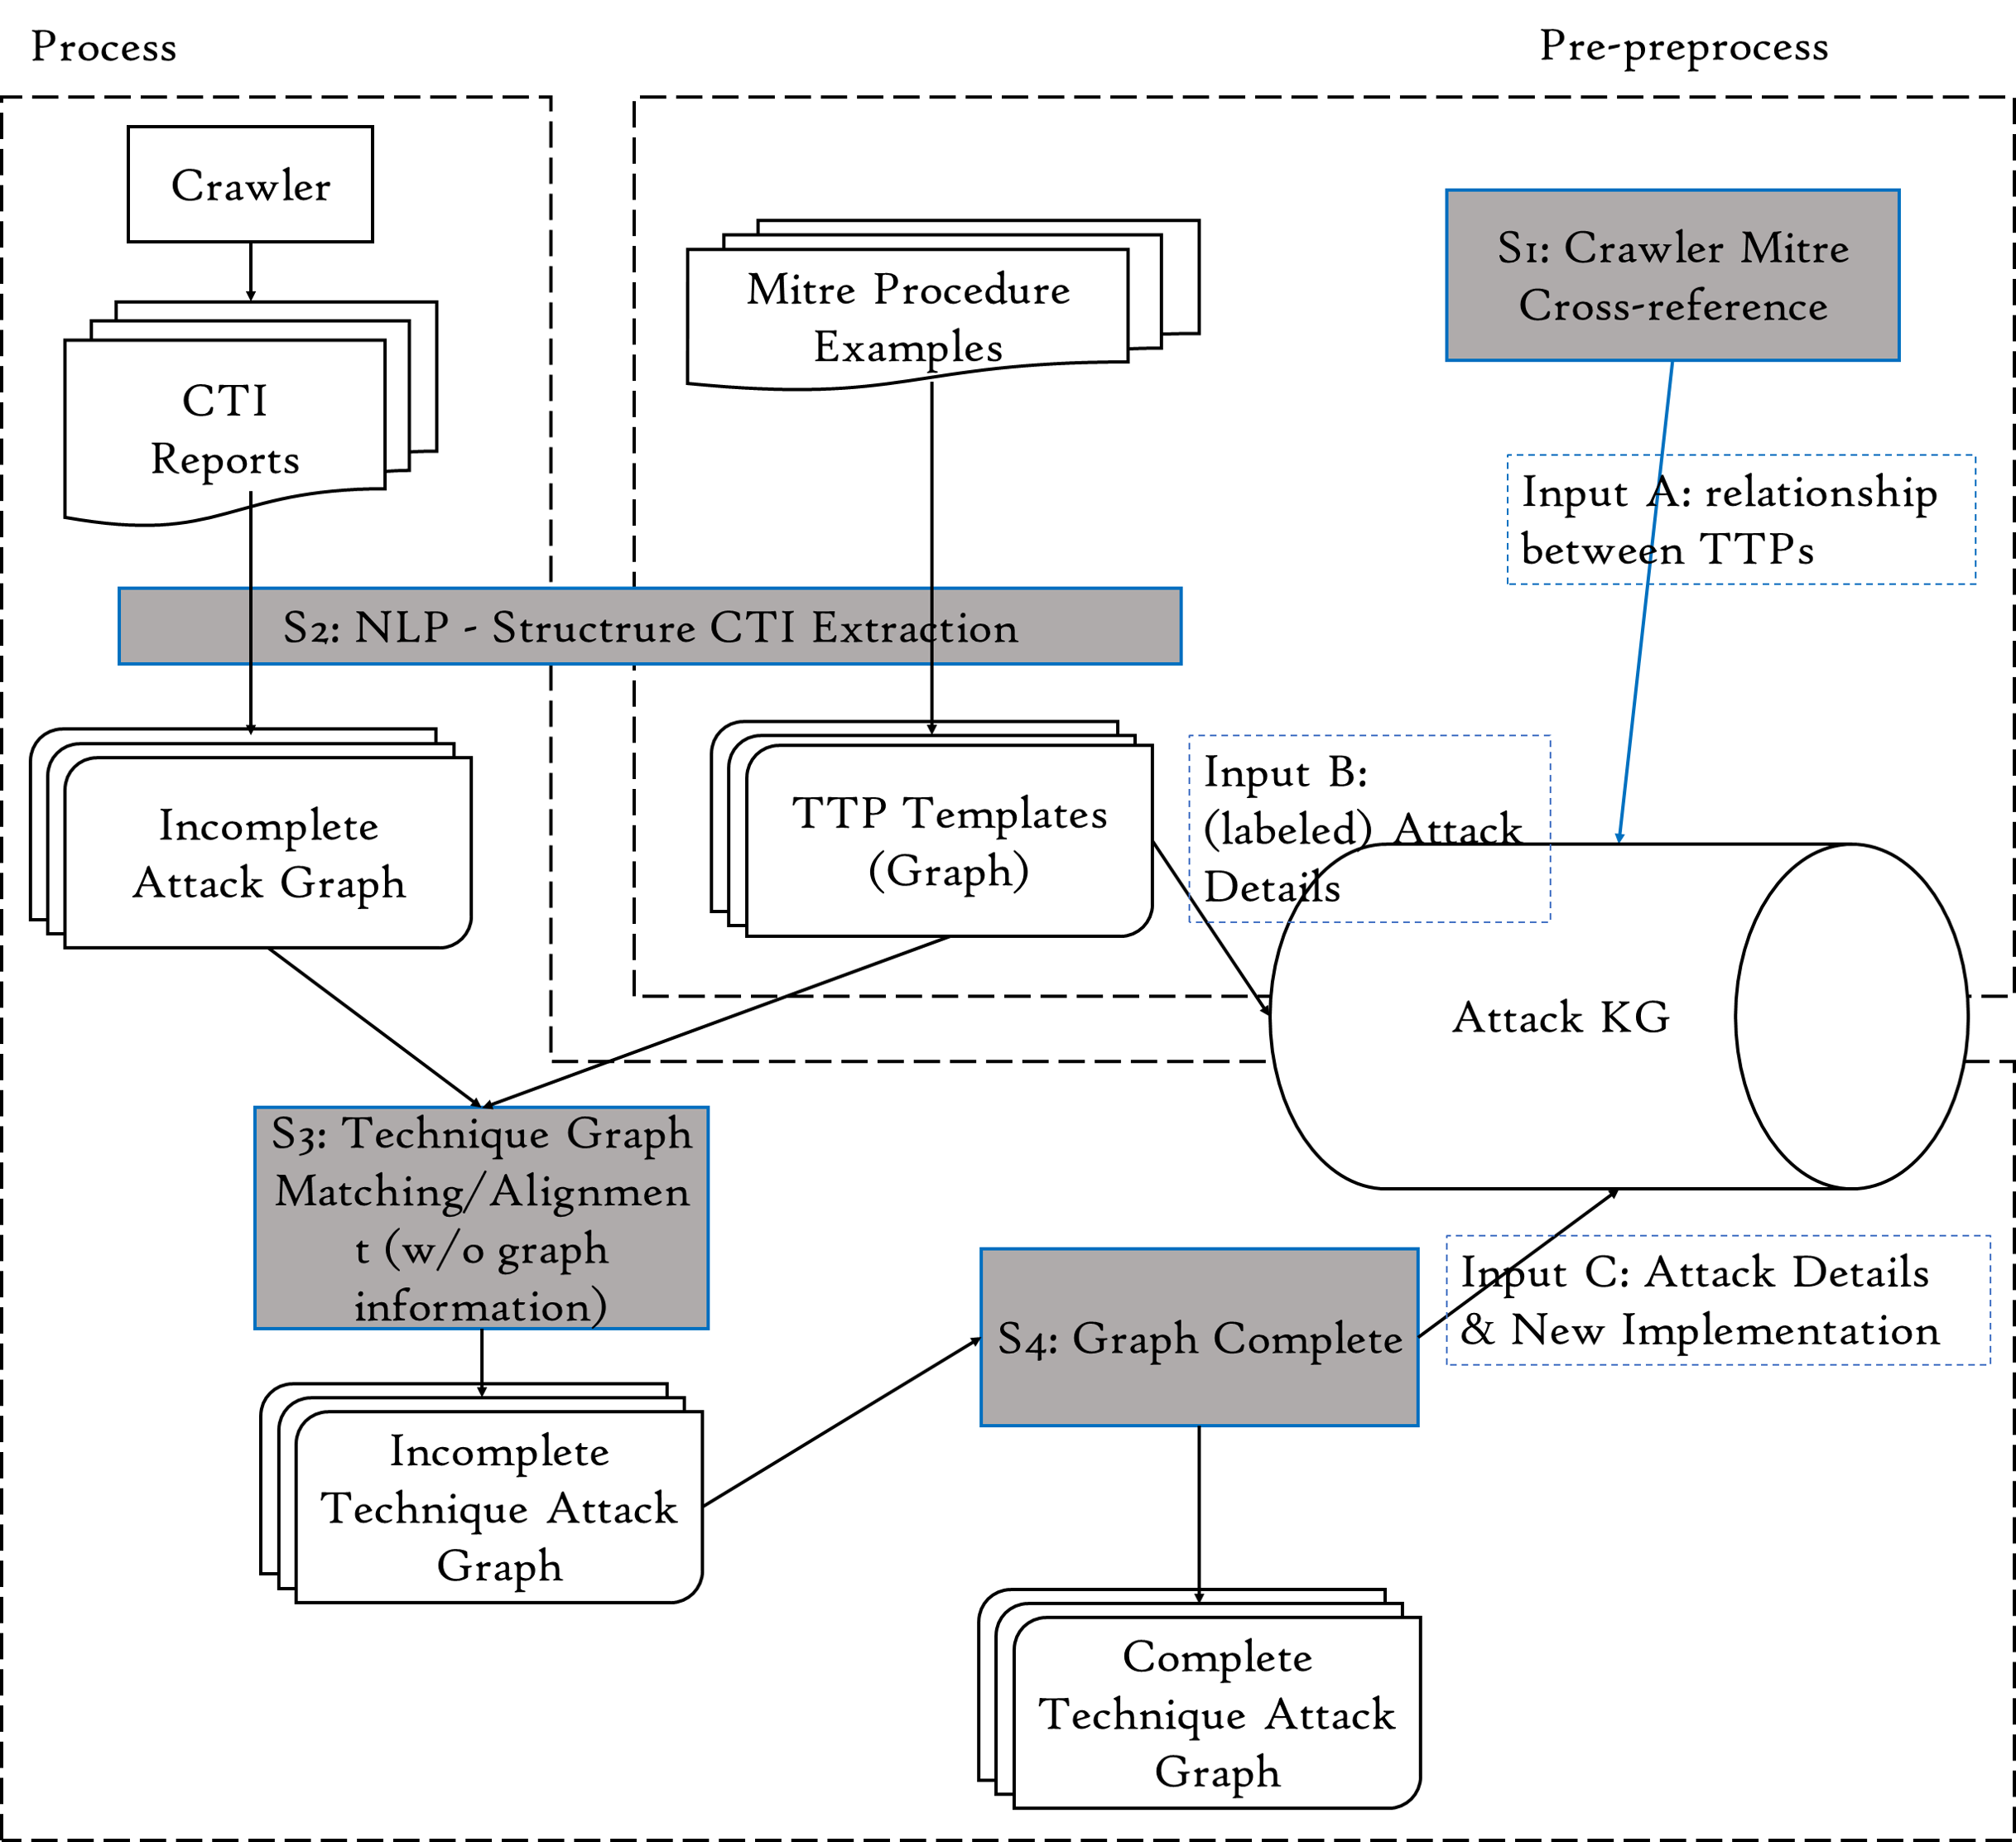
\includegraphics[width=3.3in]{Image/architecture.png}
    \caption{Attack Knowledge Graph Building Process.}
    \label{fig:architecture}
\end{figure}

\subsubsection{NLP-based CTI report parsing: the input is CTI reports and description for all the TTPs (mitre attack)}
\label{sub_sec:nlp_parser}

\begin{figure}
    \centering
    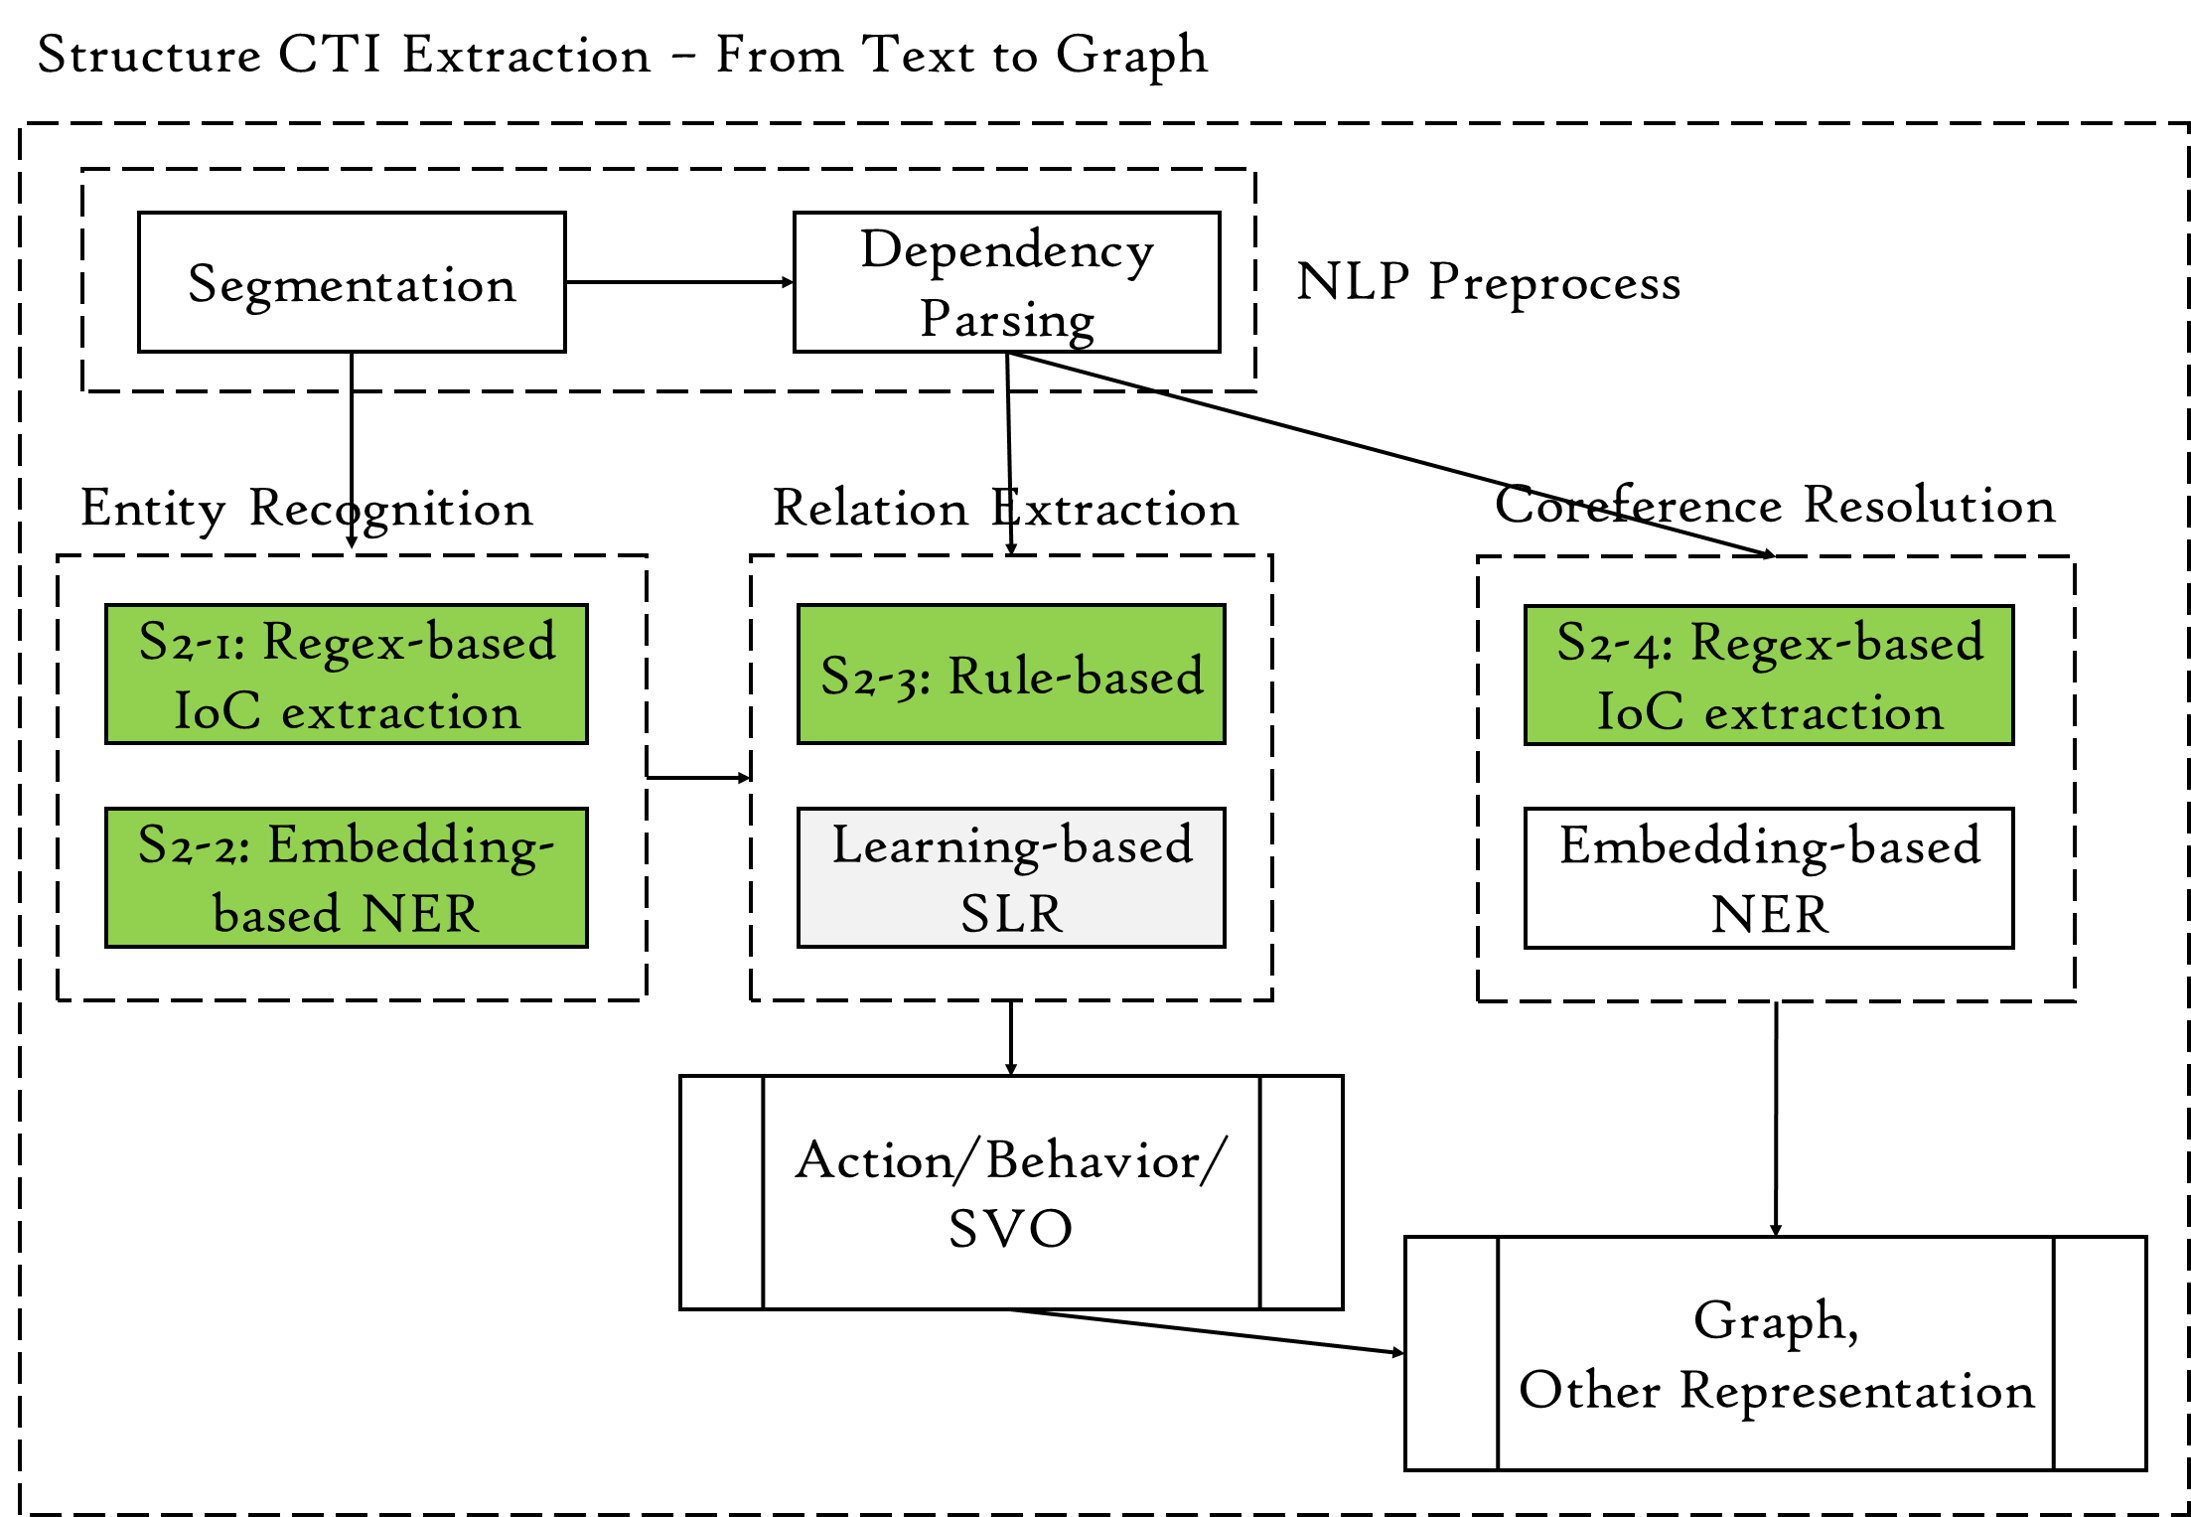
\includegraphics[width=3.3in]{Image/nlp_architecture.png}
    \caption{NLP-based Report Parsiing Process.}
    \label{fig:nlp_architecture}
\end{figure}

\ToDo{S2-0. Preprocess}

\ToDo{S2-1,2. NLP-based TTP extraction}

\ToDo{S2-3. Relation extraction}

\ToDo{S2-4. Co-reference resolution}

\ToDo{S2-5. Attack graph reconstruction for each TTP segment}

\subsubsection{TKG initialization-update-loop: the input is subgraphs representing TTPs}
\label{sub_sec:TKG_update}


\ToDo{1 Find similar subgraphs in TKG according to TTP, input/output, IoCs, subgraph structure.}

\ToDo{2 If not match, add subgraphs to the TKG; If match, find the difference and try to abstract a more general model to match both graph.}

\ToDo{3 Try to connect the new TTP with other TTPs according to the inputs and outputs.}

\subsection{TKG matching}
\label{sub_sec:matching}

\ToDo{Speed up the matching process by key nodes matching.}
